\chapter{Symmetry, Degeneracy, and Angular Momentum for Quantum Rotational Systems}

This chapter develops a symmetry-first view of rotational quantum systems. We define symmetries as operators commuting with the Hamiltonian, distinguish generic level coincidences from symmetry-protected multiplets, and build angular-momentum structure from the commutator algebra of generators. The particle on a circle provides an explicit worked model where quantized \(m\)-values, reflection pairing, and ladder operators emerge from operator algebra rather than ad hoc assumptions.

\section{Symmetry as an invariance principle}
A symmetry is an operation that leaves the quantum description unchanged. For a unitary transformation \(S\), invariance of dynamics is the condition
\[
S H S^\dagger = H
\]
equivalently
\[
[H,S]=0.
\]
Because \(S\) commutes with \(H\), Schr\"odinger evolution is covariant under \(S\): if \(|\psi(t)\rangle\) evolves by \(H\), then \(S|\psi(t)\rangle\) evolves in the same way. In particular, \(E\)-eigenvalues are mapped to the same \(E\)-eigenspaces.

Symmetries can be exact (invariance of the full Hamiltonian), approximate (effective in a regime), or accidental (valid only for very specific parameter choices). Our focus is on exact symmetries because they control spectral structure.

\section{Symmetry examples and the organizing role of operators}
The same formal rule \([H,S]=0\) unifies many familiar examples:
\begin{itemize}
\item spatial translations and rotations,
\item interchange of identical particles,
\item relabeling symmetries of a periodic lattice (discrete translation in crystal index),
\item discrete mirror or inversion operations.
\end{itemize}

In practice, this is less about geometry alone and more about algebraic leverage: a set of commuting operators gives you a good quantum-number basis, while noncommuting families often generate nontrivial multiplets. Symmetry language gives a compact way to classify allowed degeneracies before solving differential equations.

\begin{figure}[h]
\centering

\includegraphics[width=0.94\textwidth]{lecture_02_figure_01_crystal_translation.png}
\caption{Discrete translation and relabeling symmetry on an idealized crystal lattice, one of the lecture's opening examples of an operation that leaves the energy spectrum unchanged.}
\end{figure}

\section{Degeneracy, symmetry, and when degeneracy is protected}
For a bounded discrete spectrum, exact equality of two nearby energies is rare unless there is structure behind it. We call this \emph{accidental} coincidence when no symmetry explanation exists. In contrast, symmetry-protected degeneracies are stable under small perturbations that preserve the same symmetry.

\begin{proposition}
Let \(A\) and \(B\) be Hermitian symmetry generators commuting with \(H\): \([A,H]=[B,H]=0\). Define
\[
C := \frac{1}{i\hbar}[A,B].
\]
Then \(C\) is Hermitian and \([C,H]=0\).
\end{proposition}
\begin{proof}
Since \(A\) and \(B\) are Hermitian, \([A,B]^\dagger=-[A,B]\), so \(C\) is Hermitian. Then
\[
[C,H]=\frac{1}{i\hbar}\big([AB,H]-[BA,H]\big)
\]
and expanding each commutator gives zero because both \(A\) and \(B\) commute with \(H\). Hence \([C,H]=0\).
\end{proof}

Thus one can grow a closed set of symmetry generators by commutators. If that set closes to a Lie algebra with nontrivial structure constants, the representation theory is what drives degeneracy and spectral multiplets.

\section{Particle on a circle: quantized \(L_z\) from single-valued wave functions}
Let \(\theta\in[0,2\pi)\) label the position of a particle constrained to a circle. A small rotation by \(\epsilon\) acts as
\[
(\mathcal R(\epsilon)\psi)(\theta)=\psi(\theta-\epsilon).
\]
Its infinitesimal form defines the generator \(L_z\):
\[
\mathcal R(\epsilon)\psi(\theta)\approx \left(1-\frac{i\epsilon}{\hbar}L_z\right)\psi(\theta),
\qquad
L_z=-i\hbar\frac{d}{d\theta}.
\]
Hence
\[
L_z\ket{\psi_m}=m\hbar\ket{\psi_m}
\quad\Longleftrightarrow\quad
-i\hbar\frac{d\psi_m}{d\theta}=m\hbar\psi_m
\]
and therefore
\[
\psi_m(\theta)=\frac{1}{\sqrt{2\pi}}e^{im\theta}.
\]
Single-valuedness on \(0\sim 2\pi\) gives
\[
\psi_m(\theta+2\pi)=\psi_m(\theta)
\iff
e^{i2\pi m}=1
\iff
m\in\mathbb Z.
\]
So the orbital angular-momentum quantum numbers are \(m=0,\pm1,\pm2,\ldots\).

\begin{figure}[h]
\centering
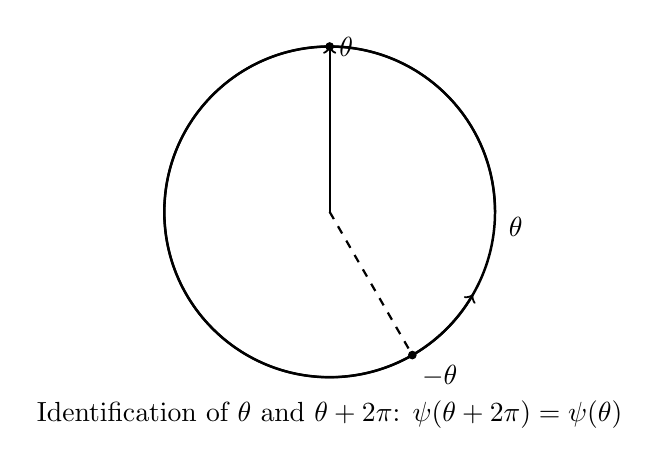
\begin{tikzpicture}[scale=1.05]
  \draw[line width=0.9pt] (0,0) circle(2.0);
  \draw[->, thick] (2,0) arc(0:330:2 and 2);
  \node at (2.25,-0.18) {$\theta$};
  \fill (90:2) circle(1.5pt) node[right] {$\theta$};
  \fill (-60:2) circle(1.5pt) node[below right] {$-\theta$};
  \draw[thick,->] (0,0) -- (90:2);
  \draw[thick,dashed] (0,0) -- (-60:2);
  \node at (0,-2.45) {Identification of \(\theta\) and \(\theta+2\pi\): \(\psi(\theta+2\pi)=\psi(\theta)\)};
\end{tikzpicture}
\caption{Circle coordinate, opposite angles, and periodicity condition.}
\end{figure}

\section{Mirror symmetry and the \(m\leftrightarrow -m\) pairing}
Introduce a mirror (reflection) operator \(\mathcal M\) with
\[
(\mathcal M\psi)(\theta)=\psi(-\theta).
\]
Its action on a momentum eigenmode is
\[
\mathcal M\psi_m(\theta)=\psi_{-m}(\theta).
\]
On a circle eigenstate:
\[
\mathcal M L_z\psi_m = m\hbar\,\mathcal M\psi_m,\qquad
L_z\mathcal M\psi_m = -m\hbar\,\mathcal M\psi_m,
\]
so
\[
[\mathcal M,L_z]\psi_m = 2m\hbar\,\mathcal M\psi_m\neq 0\quad (m\neq0).
\]
Thus \(\mathcal M\) does not commute with \(L_z\), even though both may commute with \(H\) in a symmetric setup. When both symmetries are present (no mirror-breaking field), states \(m\) and \(-m\) are paired at equal energy.

Important warning from the formalism: equal probabilities \(|\psi_m(\theta)|^2=|\psi_{-m}(\theta)|^2\) does not imply identical wave functions. Degeneracy concerns states and operators, not only densities.

A uniform magnetic field is a standard counterexample: it can split \(\pm m\) levels while preserving some rotational structure of orbital motion in other settings. Symmetry arguments apply to what the Hamiltonian does, not to geometric intuition alone.

\section{Generators, commutator algebra, and closure}
For continuous symmetries a small transformation is written as
\[
U(\epsilon)=1-\frac{i\epsilon}{\hbar}G+\mathcal O(\epsilon^2),
\]
with Hermitian generator \(G\). The commutator of two generators is another generator of another direction in the same symmetry structure if closure holds.

A useful worked pattern is:
\[
\begin{aligned}
[\,\mathcal M,L_z\,]&\neq 0,\\
[H,L_z]&=0,\qquad [H,\mathcal M]=0
\quad(\text{if mirror symmetric}).
\end{aligned}
\]
Hence \(\mathcal M\) and \(L_z\) generate two operations whose noncommutativity forces additional structure.

\section{Three-dimensional angular momentum and ladder structure}
For a particle in 3D,
\[
\begin{aligned}
L_x&= y p_z-z p_y,\\
L_y&= z p_x-x p_z,\\
L_z&= x p_y-y p_x.
\end{aligned}
\]
with canonical \([x_i,p_j]=i\hbar\delta_{ij}\). A compact expansion gives
\[
[L_x,L_y]=i\hbar L_z,
\]
and cyclic permutations. Equivalently,
\[
[L_i,L_j]=i\hbar\sum_k \epsilon_{ijk}L_k.
\]
For a rotationally invariant Hamiltonian, \([H,L_i]=0\), so \(L_x,L_y,L_z\) are conserved quantities.

Define raising and lowering operators
\[
L_\pm:=L_x\pm iL_y.
\]
Using the algebra above,
\[
[L_z,L_\pm]=\pm\hbar L_\pm,\qquad [L_+,L_-]=2\hbar L_z.
\]
If \(|\ell,m\rangle\) is an eigenvector of \(L_z\),
\[
L_z|\ell,m\rangle=m\hbar|\ell,m\rangle,
\]
then
\[
L_z(L_\pm|\ell,m\rangle)=(m\pm1)\hbar (L_\pm|\ell,m\rangle),
\]
so \(L_\pm\) create a state with adjacent \(m\)-value when nonzero.

In a finite ladder representation, the chain terminates:
\[
L_+|\ell,\ell\rangle=0,\qquad L_-|\ell,-\ell\rangle=0,
\]
giving \(m=-\ell,-\ell+1,\ldots,\ell\), hence \(2\ell+1\) states in one rotational multiplet. For orbital wave functions on configuration space, \(\ell,m\in\mathbb Z\) and \(m\in\{-\ell,\ldots,\ell\}\). For more general angular-momentum types (including spin), half-integer \(m\) spectra are also possible; in this lecture the orbital circle argument selects the integer branch.

\begin{figure}[h]
\centering

\includegraphics[width=0.74\textwidth]{lecture_02_frame_05.png}
\caption{Illustrative ladder picture: \(L_\pm\) connect adjacent \(m\)-levels inside a symmetry multiplet.}
\end{figure}

\section{Summary}
Symmetry enters as a commutation criterion with the Hamiltonian. Single symmetries can explain invariant spectral structure, but genuine multiplets require a noncommuting symmetry set whose commutator algebra closes. The circle provides the cleanest demonstration: rotational invariance gives \(L_z=-i\hbar\partial_\theta\), single-valuedness gives integer \(m\), and mirror symmetry links \(m\) to \(-m\). In three dimensions, the algebra \([L_i,L_j]=i\hbar\epsilon_{ijk}L_k\) yields ladder operators \(L_\pm\), a finite \(m\)-tower for each \(\ell\), and equal-energy multiplets in rotationally invariant systems.
